% Ekdant -- MSc thesis progress report (2026-11-11)
% Build: tectonic Ekdant_Progress_Report.tex   (XeLaTeX engine)
% Every number comes from run.md (A2, A3o-A3s, A7k-A7n), the gain_*.md /
% reason_*.md reports in 09-Code, and the code / config of the final model.
\documentclass[a4paper,11pt,parskip=half]{scrartcl}

\usepackage{fontspec}
\usepackage{amsmath,amssymb}
\usepackage[a4paper,margin=2.4cm,top=2.6cm,bottom=2.8cm]{geometry}
\usepackage{graphicx}
\usepackage{float}
\usepackage{booktabs,tabularx,array,multirow}
\usepackage{xcolor}
\usepackage{tikz}
\usetikzlibrary{arrows.meta,positioning,calc,fit,backgrounds,shapes.geometric}
\usepackage[font=small,labelfont=bf,margin=0.5cm]{caption}
\usepackage{enumitem}
\usepackage[most]{tcolorbox}
\usepackage{microtype}
\usepackage[hidelinks]{hyperref}
\usepackage{scrlayer-scrpage}

\definecolor{lblue}{HTML}{2A78D6}
\definecolor{lsoft}{HTML}{E6F0FB}
\definecolor{lorange}{HTML}{EB6834}
\definecolor{lgreen}{HTML}{1F7A46}
\definecolor{ink}{HTML}{17191C}
\definecolor{muted}{HTML}{575B62}
\definecolor{rule}{HTML}{DEDFDC}

\addtokomafont{disposition}{\color{ink}}
\addtokomafont{section}{\Large}
\setlist{itemsep=2pt,topsep=3pt}
\renewcommand{\arraystretch}{1.18}
\newcolumntype{Y}{>{\raggedright\arraybackslash}X}
\newcolumntype{R}{>{\raggedleft\arraybackslash}X}

\newcommand{\sig}{\ensuremath{^{\ast}}}
\newcommand{\Ltwo}{L2}
\newcommand{\code}[1]{\texttt{\small #1}}

\newtcolorbox{keybox}[1][]{enhanced,colback=lsoft,colframe=lblue,boxrule=0.6pt,
  arc=2pt,left=8pt,right=8pt,top=6pt,bottom=6pt,fonttitle=\bfseries,#1}
\newtcolorbox{rulebox}[1][]{enhanced,colback=white,colframe=ink,boxrule=0.5pt,
  arc=2pt,left=8pt,right=8pt,top=6pt,bottom=6pt,fonttitle=\bfseries,
  colbacktitle=ink!8,coltitle=ink,#1}

\pagestyle{scrheadings}
\clearpairofpagestyles
\ihead{\small\color{muted}Ekdant -- progress report}
\ohead{\small\color{muted}11 November 2026}
\cfoot{\small\pagemark}

\tikzset{
  >={Stealth[length=2.4mm]},
  blk/.style={draw=ink,thick,rounded corners=3pt,fill=white,align=center,
              minimum height=1.1cm,inner sep=4pt,font=\small},
  l2blk/.style={blk,draw=lblue,fill=lsoft,very thick},
  stage/.style={draw=ink,rounded corners=3pt,fill=white,thick},
  lane/.style={lblue,line width=1.3pt},
  lab/.style={font=\footnotesize,color=muted,align=center},
  flow/.style={->,thick,ink},
  bflow/.style={->,very thick,lblue},
}

\hypersetup{pdftitle={Ekdant: progress report on the L2 add-on},
  pdfauthor={Harshil Gorasiya}}

% =====================================================================
\begin{document}

\begin{titlepage}
  \thispagestyle{empty}
  \vspace*{2.2cm}
  {\color{muted}\large\sffamily MSc thesis \textbullet{} Hochschule Heilbronn}\par
  \vspace{0.6cm}
  {\color{ink}\fontsize{26}{31}\selectfont\sffamily\bfseries Can an internal ``debate'' add-on\\[2pt] make a small language model\\[2pt] reason better?\par}
  \vspace{0.6cm}
  {\Large\sffamily\color{lblue} Progress report on the L2 add-on (project Ekdant)\par}
  \vspace{1.4cm}
  \begin{tikzpicture}
    \draw[lblue,line width=2pt] (0,0) -- (14,0);
  \end{tikzpicture}\par
  \vspace{0.8cm}
  {\large\sffamily Harshil Gorasiya\par}
  \vspace{0.2cm}
  {\sffamily\color{muted} Status: 11 November 2026\par}
  \vfill
  \begin{keybox}[title={In one paragraph}]
  L2 is a 19.6\,M-parameter add-on attached to the pretrained language model
  SmolLM2-135M. It runs four internal candidate states (``trajectories'') of
  each token, lets them debate and averages them. Over nine L2 versions, three
  training seeds per final model and three purpose-built reasoning tests,
  \textbf{L2 never showed better reasoning}. Its best accuracy gain
  (+2.07\sig{} points on PubMedQA) turned out to be a preference for answering
  ``yes''. The positive results of the project are a \textbf{data finding}
  (training the yes/no decision from the evidence: PubMedQA
  58.0\,\% $\rightarrow$ 61.3\,\% without any add-on) and an
  \textbf{evaluation method} that separates reasoning from answer preference.
  \end{keybox}
  \vspace{0.4cm}
  {\footnotesize\color{muted} All numbers are means over seeds 17, 23 and 31. Differences carry a paired bootstrap 95\,\% confidence interval; \sig{} marks an interval that excludes 0. Accuracy differences are in percentage points.\par}
\end{titlepage}

\tableofcontents
\vspace{1em}

\begin{rulebox}[title={Findings at a glance}]
\begin{tabularx}{\linewidth}{@{}p{3.3cm}Y@{}}
\textbf{\color{lgreen}Worked} & \textbf{Training the decision from the evidence (T61).} PubMedQA 58.0 $\rightarrow$ 61.3\,\%\sig{} without any add-on; following flipped evidence 27\,\% $\rightarrow$ 79--80\,\%; 3-benchmark average +1.25\sig; a fifth of the training text.\\[3pt]
\textbf{\color{lgreen}Worked} & \textbf{Three reasoning tests + L2-off test.} They exposed L2's +2-point PubMedQA gain as a ``yes'' preference (+11.0\sig{} more ``yes'' answers), which accuracy alone hides.\\[3pt]
\textbf{\color{lorange}Not useful} & \textbf{The L2 layer.} Reasoning never shown; with the right data it adds $-0.10$ points; text perplexity drops by under 2\,\% but the generated text is no better.
\end{tabularx}
\end{rulebox}

% =====================================================================
\section{The question}

Small language models answer medical questions largely by pattern matching.
The idea behind this thesis is to add a separate ``thinking'' module on top of
an ordinary language model. Inside it, several candidate versions of the
model's internal state -- \emph{trajectories} -- start from different angles,
read each other, revise themselves and agree on one answer state: a small
internal debate inside a single forward pass, without generating extra text.

The original design had two parts, L1 and L2. L1 is left for future work;
this thesis tests \textbf{L2 alone}, on a pretrained model, against the same
model without it.

\begin{keybox}[title={Research question}]
Does SmolLM2 + L2 \emph{reason} better on medical question answering than
SmolLM2 alone, when both are trained on exactly the same data? ``Reason
better'' must mean more than higher accuracy; Section~\ref{sec:eval} defines
how it is tested.
\end{keybox}

% =====================================================================
\section{The model}

\subsection{The backbone: SmolLM2-135M}

SmolLM2-135M~\cite{smollm2} is a public, pretrained, decoder-only language
model whose task is to predict the next token. All of its weights are
fine-tuned (full fine-tuning); LoRA was tried only as one variant (T60).

\begin{table}[H]
\centering\small
\begin{tabularx}{0.9\linewidth}{@{}lY@{}}
\toprule
Property & Value\\
\midrule
Parameters & 134{,}515{,}584 ($\approx$ 135\,M)\\
Layers & 30 decoder layers (self-attention + MLP), RMSNorm~\cite{rmsnorm}, rotary position encoding\\
Hidden size & 576 numbers per token -- the token's \emph{state} $h$\\
Attention & 9 query heads, 3 key/value heads (grouped-query attention)\\
Vocabulary & 49{,}152 tokens; output layer (\code{lm\_head}) tied to the input embedding\\
Context used & up to 1{,}024 tokens per example (answers up to 512)\\
\bottomrule
\end{tabularx}
\caption{The backbone.}
\end{table}

\subsection{Where L2 attaches}

In the final model (v5), L2 sits between SmolLM2's last layer and its output
layer (Figure~\ref{fig:whole}). For every token, SmolLM2 produces a final state
$h\in\mathbb{R}^{576}$. L2 computes a refined state $y$, and a learned
per-channel gate $g$ decides how much of $y$ replaces $h$:
\begin{equation}
  h' = h + g \odot (y - h), \qquad g = \tanh(\gamma_{\text{gate}}) \in \mathbb{R}^{576}, \quad \gamma_{\text{gate}} = 0 \text{ at the start.}
  \label{eq:gate}
\end{equation}
Because the gate starts at 0, the model at step 0 \emph{is} SmolLM2; any
difference between the two arms is learned. In trained v5 the gates end at
$|g| \approx 0.025$--$0.028$, i.e.\ L2 replaces roughly 3\,\% of the final state.

\begin{figure}[H]
\centering
\resizebox{\linewidth}{!}{\begin{tikzpicture}[node distance=0.9cm]
  \node[blk,minimum width=2.1cm] (p) {\textbf{Prompt}\\[-1pt]{\scriptsize\color{muted}question (+ abstract)}};
  \node[blk,right=1.1cm of p,minimum width=2.8cm,minimum height=1.5cm] (s) {\textbf{SmolLM2-135M}\\30 decoder layers\\+ final RMSNorm};
  \coordinate[right=0.7cm of s] (sp);
  \node[l2blk,right=0.6cm of sp,minimum width=2.7cm,minimum height=1.4cm] (l2) {\textbf{L2}\\{\footnotesize 4 trajectories, debate,}\\{\footnotesize descent, average}};
  \node[circle,draw=ink,thick,minimum size=0.85cm,right=0.9cm of l2] (g) {$g$};
  \node[blk,right=0.8cm of g,minimum width=1.9cm] (head) {\textbf{lm\_head}\\[-1pt]{\scriptsize\color{muted}49,152 words}};
  \node[right=0.5cm of head,font=\small\bfseries,align=center] (o) {next\\word};
  \draw[flow] (p) -- node[above,lab]{tokens} (s);
  \draw[thick] (s) -- node[above,font=\small]{$h$} (sp);
  \fill (sp) circle (2pt);
  \draw[bflow] (sp) -- (l2);
  \draw[bflow] (l2) -- node[above,font=\small]{$y$} (g);
  \draw[flow] (sp) -- ++(0,1.5) -| node[pos=0.25,above,lab]{skip path: $h$ unchanged} (g);
  \draw[flow] (g) -- node[above,font=\small]{$h'$} (head);
  \draw[flow] (head) -- (o);
  \node[below=0.35cm of g,font=\small,align=center] {$h' = h + g\odot(y-h)$\\[-1pt]{\scriptsize\color{muted}576 gates, start at 0; trained: $|g|\approx 0.027$}};
\end{tikzpicture}}
\caption{The whole model. SmolLM2 produces the state $h$ of every token. $h$ goes both into L2 and, unchanged, along the skip path. The gate mixes the two before the output layer predicts the next word. $y=\mathrm{RMSNorm}(c)$, where $c$ is L2's consensus state (Figure~\ref{fig:inside}).}
\label{fig:whole}
\end{figure}

% =====================================================================
\section{The L2 layer in detail}
\label{sec:l2}

L2 works on \textbf{one token at a time}. It takes that token's final state
$h$ and runs four steps: \emph{diverse start} $\rightarrow$ \emph{4 debate
rounds} $\rightarrow$ \emph{8 anchored descent steps} $\rightarrow$
\emph{average} (Figure~\ref{fig:inside}). All settings are those of the final
model v5 (\code{configs/v5\_final.json}; code in
\code{09-Code/src/ekdant/sandbox.py} and \code{model.py}).

\begin{figure}[H]
\centering
\resizebox{\linewidth}{!}{\begin{tikzpicture}[x=1cm,y=1cm]
  % input
  \node[blk,minimum width=1.0cm] (h) at (0,0) {$h$\\[-2pt]{\scriptsize\color{muted}576}};
  % stage boxes
  \draw[stage] (1.2,-2.6) rectangle (3.8,2.9);
  \draw[stage] (4.4,-2.6) rectangle (9.2,2.9);
  \draw[stage] (9.8,-2.6) rectangle (14.0,2.9);
  \node[font=\footnotesize\bfseries] at (2.5,2.45) {1 \textperiodcentered{} Start};
  \node[lab,font=\scriptsize] at (2.5,2.05) {4 views of $h$};
  \node[font=\footnotesize\bfseries] at (6.8,2.45) {2 \textperiodcentered{} Debate, 4 rounds};
  \node[lab,font=\scriptsize] at (6.8,2.05) {own weights per round};
  \node[font=\footnotesize\bfseries] at (11.9,2.45) {3 \textperiodcentered{} Descent, 8 steps};
  \node[lab,font=\scriptsize] at (11.9,2.05) {pull towards anchor $a$};
  \node[font=\footnotesize\bfseries] at (15.4,2.45) {4 \textperiodcentered{} Average};
  \draw[flow] (h.east) -- (1.2,0);
  % lanes
  \foreach \y/\k in {1.4/1,0.47/2,-0.47/3,-1.4/4} {
    \node[font=\small] at (2.5,\y) {$T_{\k}$};
    \draw[lane] (3.0,\y) -- (14.4,\y) -- (15.0,0);
  }
  % cross reads
  \draw[<->,lblue,dashed,thick] (5.4,1.32) -- (5.4,0.55);
  \draw[<->,lblue,dashed,thick] (6.3,0.39) -- (6.3,-0.39);
  \draw[<->,lblue,dashed,thick] (7.2,-0.55) -- (7.2,-1.32);
  \draw[<->,lblue,dashed,thick] (8.1,1.32) to[bend left=35] (8.1,-1.32);
  % mean
  \node[circle,draw=lblue,fill=lsoft,very thick,minimum size=0.75cm] (m) at (15.2,0) {$\bar{x}$};
  \draw[flow] (m.east) -- (16.3,0) node[right,font=\small,align=center] {$c$\\[-2pt]{\scriptsize\color{muted}576}};
  % bottom labels
  \node[lab,font=\scriptsize] at (2.5,-2.15) {$T_k = W_k h + b_k$};
  \node[lab,font=\scriptsize] at (6.8,-2.15) {each $T_k$ reads the other 3};
  \node[lab,font=\scriptsize] at (11.9,-2.15) {$T_k \leftarrow T_k - \eta\, s_k \odot (T_k - a)$};
  % anchor
  \draw[->,thick,dashed,ink] (h.south) -- (0,-3.3) -- node[below,lab]{anchor $a = W_a h$, computed from the same $h$} (11.9,-3.3) -- (11.9,-2.6);
\end{tikzpicture}}
\caption{Inside L2, for one token. Blue lines are the four trajectories; dashed blue arrows are the cross-reads in every debate round; the dashed black line is the anchor, computed from the same input $h$. The output $c$ is L2's consensus state.}
\label{fig:inside}
\end{figure}

\begin{figure}[H]
\centering
\resizebox{\linewidth}{!}{\begin{tikzpicture}[x=1cm,y=1cm]
  \node[font=\small] (t) at (0,0) {$T_k$};
  \node[blk,minimum width=1.7cm] (n) at (1.9,0) {RMSNorm};
  \coordinate (xk) at (3.6,0);
  \node[l2blk,minimum width=2.7cm] (cr) at (6.0,0) {\textbf{Cross-read}\\[-1pt]{\scriptsize attention over $x_j$, $j\neq k$}};
  \coordinate (ck) at (8.4,0);
  \node[blk,minimum width=2.7cm] (mlp) at (11.0,0) {\textbf{MLP}\\[-1pt]{\scriptsize 576$\rightarrow$2304$\rightarrow$576, SiLU}};
  \node[blk,minimum width=2.7cm] (gt) at (11.0,-2.2) {\textbf{Repair gate} $\gamma_k$\\[-1pt]{\scriptsize $\sigma(W_\gamma[x_k;\mathrm{cross}_k]+b_\gamma)$}};
  \node[circle,draw=ink,thick,minimum size=0.9cm,font=\small] (mix) at (14.9,0) {mix};
  \node[font=\small,align=center] (out) at (17.1,0) {new $T_k$\\[-1pt]{\scriptsize $(1-\gamma_k)\odot T_k$}\\[-3pt]{\scriptsize $+\,\gamma_k\odot$ proposal}};
  \draw[flow] (t) -- (n);
  \draw[flow] (n) -- node[above,font=\small]{$x_k$} (cr);
  \draw[flow] (cr) -- node[above,font=\small]{cross$_k$} (mlp);
  \draw[flow] (mlp) -- node[above,lab]{proposal} (mix);
  \draw[flow] (mix) -- (out);
  \draw[->,thick,dashed] (6.0,-1.45) node[left,lab,align=right]{other 3\\trajectories} -- (cr.south);
  \draw[flow] (xk) |- ([yshift=-6pt]gt.west);
  \draw[flow] (ck) |- ([yshift=6pt]gt.west);
  \draw[flow] (gt.east) -| node[pos=0.75,right,font=\small]{$\gamma_k$} (mix.south);
  \draw[flow] (0.45,0) -- (0.45,1.3) -| node[pos=0.25,above,lab]{old state $T_k$ (kept where $\gamma_k$ is small)} (mix.north);
\end{tikzpicture}}
\caption{One debate round, for trajectory $k$. The repair gate $\gamma_k$ lets a trajectory keep its own state instead of following the others. Its bias starts at $-2$, so initially $\gamma_k \approx 0.12$ and each round changes little.}
\label{fig:round}
\end{figure}

\subsection{The computation, step by step}

Let $h \in \mathbb{R}^{576}$ be the final state of one token, $K=4$ trajectories, $R=4$ debate rounds, $S=8$ descent steps.

\paragraph{1. Diverse start.} For $k=1,\dots,K$:
\begin{equation}
  T_k = W_k h + b_k ,
\end{equation}
where $W_1,\dots,W_4 \in \mathbb{R}^{576\times576}$ are initialised mutually orthogonal (Frobenius inner product 0) with gains spread logarithmically from 0.8 to 1.25. The four trajectories therefore begin as four different ``views'' of $h$.

\paragraph{2. Debate rounds} ($r=1,\dots,R$, each with its own weights):
\begin{align}
  x_k &= \mathrm{RMSNorm}(T_k),\\
  \mathrm{cross}_k &= \sum_{j\neq k} \operatorname{softmax}_j\!\left(\frac{(Q x_k)^{\!\top}(K x_j)}{\sqrt{576}}\right) V x_j,\\
  \gamma_k &= \sigma\big(W_\gamma [x_k ; \mathrm{cross}_k] + b_\gamma\big), \qquad b_\gamma = -2 \text{ at init},\\
  T_k &\leftarrow (1-\gamma_k)\odot T_k + \gamma_k \odot \mathrm{MLP}(\mathrm{cross}_k).
\end{align}
The attention runs \emph{across trajectories of the same token} (never across tokens), and a trajectory never attends to itself.

\paragraph{3. Anchored descent} ($S=8$ steps, $\eta = 0.0625$):
\begin{align}
  a &= W_a h, \\
  T_k &\leftarrow T_k - \eta\; \sigma\big(W_s [T_k ; a]\big) \odot (T_k - a).
\end{align}

\paragraph{4. Consensus and output.}
\begin{equation}
  c = \frac{1}{K}\sum_{k=1}^{K} T_k, \qquad y = \mathrm{RMSNorm}(c), \qquad h' = h + g\odot(y-h), \qquad \text{logits} = \mathrm{lm\_head}(h').
\end{equation}

\paragraph{Training loss.} Next-token cross-entropy on the answer tokens plus a \emph{spread floor} that keeps the trajectories apart:
\begin{equation}
  \mathcal{L} = \mathcal{L}_{\text{CE}} + \lambda\, \max(0,\ \rho_{\min} - \rho)^2, \qquad
  \rho = \frac{\operatorname{Var}_k(T_k)}{\overline{h^2}}, \quad \rho_{\min}=0.05,\ \lambda = 1 .
\end{equation}

\subsection{Why each part is there}
\begin{itemize}
  \item \textbf{Diverse start} -- if all trajectories started equal, the debate would have nothing to argue about.
  \item \textbf{Debate} -- each trajectory reads the others and proposes an update; the \textbf{repair gate} lets it decline the crowd, so a correct minority can survive a round.
  \item \textbf{Anchored descent} -- pulls every trajectory back towards an anchor computed from the original state, so the debate cannot drift away from what the model read. A second gate decides per channel how strongly to pull.
  \item \textbf{Average} -- the consensus is the plain mean (\code{readout = mean}).
  \item \textbf{Spread floor} -- without it the four trajectories could collapse into one, and L2 would be a single MLP.
  \item \textbf{Zero gate at start} -- both arms begin with exactly SmolLM2's output; the comparison is fair from step 0.
\end{itemize}

\subsection{Parameter count}

\begin{table}[H]
\centering\small
\begin{tabularx}{\linewidth}{@{}lYr@{}}
\toprule
Part & Weights & Parameters\\
\midrule
Diverse start & 4 matrices $576\times576$ + 4 biases & 1{,}329{,}408\\
One debate round & pre-norm 576; $Q,K,V$: $3\times576^2$; repair gate $1152\rightarrow576$; MLP $576\rightarrow2304\rightarrow576$ & 4{,}317{,}120\\
4 debate rounds & $4\times$ the above & 17{,}268{,}480\\
Anchored descent & anchor $576^2$; descent gate $1152\rightarrow576$ & 995{,}904\\
Output & output RMSNorm 576; gate 576 & 1{,}152\\
\midrule
\textbf{L2 total} & & \textbf{19{,}594{,}944} (+14.6\,\%)\\
SmolLM2 + L2 & & 154{,}110{,}528\\
\bottomrule
\end{tabularx}
\caption{Parameters of L2 in v5. The comparison with the baseline is architecture-matched, not parameter-matched.}
\end{table}

\subsection{What L2 can and cannot see}

\begin{keybox}[title={An important property of the final design}]
In v5, L2 works \textbf{per token}: it sees only that token's final state $h$, not the other tokens and not the abstract itself. Everything it knows about the question and the evidence is what SmolLM2 has already encoded in $h$. Because L2 sits at the very end, no later layer reads its output either. L2 can therefore only \emph{reshape} what SmolLM2 has computed; it cannot gather new evidence. Later versions (v3--v4) gave L2 its own attention over the text, a verifier, a vote and placements inside the network; none did better than v5 (Section~\ref{sec:history}).
\end{keybox}

% =====================================================================
\section{Data}
\label{sec:data}

\subsection{Datasets}

\begin{table}[H]
\centering\small
\begin{tabularx}{\linewidth}{@{}>{\raggedright\arraybackslash}p{3.1cm}Y>{\raggedright\arraybackslash}p{4.6cm}@{}}
\toprule
Dataset & Content & Use\\
\midrule
PubMedQA \code{pqa\_artificial}~\cite{pubmedqa} & 211{,}269 research questions, each with a PubMed abstract, the authors' conclusion and an automatically generated yes/no label & Training, stage 1 (2{,}000 rows held out)\\
MedQuAD~\cite{medquad} & 16{,}407 consumer-health questions with answers from NIH websites (14{,}345 unique questions) & Split by unique question: one half trains stage 2 (10\,\% of it selects the checkpoint), the other half is only a benchmark\\
PubMedQA \code{pqa\_labeled}~\cite{pubmedqa} & 1{,}000 questions with expert yes/no/maybe labels & Benchmark only; no PubMed id shared with the training set (checked)\\
\bottomrule
\end{tabularx}
\caption{Training and evaluation data. All datasets are public.}
\end{table}

\subsection{The ``old data'' (v1--v5, T59, T60)}

Stage 1 was trained as \textbf{question + abstract $\rightarrow$ write the authors' conclusion} (209{,}269 rows, about 85\,M tokens per epoch). Two problems were found:
\begin{enumerate}
  \item \textbf{The labels are 92.8\,\% ``yes''}: 196{,}144 yes, 15{,}125 no, no maybe.
  \item \textbf{The yes/no word was never a training target.} The model only learned to write the conclusion, whereas the PubMedQA benchmark scores exactly the yes/no word. The benchmark answer was therefore a side effect of conclusion writing.
\end{enumerate}
This explains how L2 could raise PubMedQA accuracy by learning to say ``yes'' more often -- the majority answer -- without reading the evidence any better.

\subsection{The evidence data (T61, \code{-{}-evidence})}

Only stage 1 is rebuilt; MedQuAD and every benchmark stay unchanged. The training answer now starts with the decision, and half of the rows force that decision to come from the evidence. The idea follows counterfactually augmented data~\cite{kaushik}.

\begin{table}[H]
\centering\small
\begin{tabularx}{\linewidth}{@{}lYYr@{}}
\toprule
Rows & Prompt & Target & Count (seed 17)\\
\midrule
Balanced & question + abstract & \code{yes. <conclusion>} or \code{no. <conclusion>} & 29{,}934\\
Flipped pairs & question + the conclusion only & \code{yes} / \code{no} & $2\times45{,}774$\\
\bottomrule
\end{tabularx}
\caption{The evidence data: 121{,}482 short rows, about a fifth of the old text (about 0.9\,h per training run).}
\end{table}

\begin{itemize}
  \item \textbf{Balanced rows:} every ``no'' row plus the same number of ``yes'' rows, so always answering ``yes'' scores only 50\,\%.
  \item \textbf{Flipped pairs:} each conclusion appears twice -- once as written with its real label, and once with one negation added or removed (e.g.\ ``does not improve'' $\leftrightarrow$ ``does improve'') with the opposite label. Only a model that actually reads the sentence gets both right.
  \item The 1{,}000 benchmark questions are excluded from training.
\end{itemize}

\subsection{The pair loss (T63, \code{-{}-pair-loss 1.0})}

With plain cross-entropy, each row of a flipped pair is trained on its own. PairCFR~\cite{paircfr} reports that counterfactual pairs help more when the loss compares both rows. Both rows of a pair are therefore placed in the same batch, and the loss adds
\begin{equation}
  \mathcal{L}_{\text{pair}} = W \cdot \operatorname{softplus}\big(m_{\text{no-row}} - m_{\text{yes-row}}\big), \qquad
  m = \operatorname{logit}(\text{``yes''}) - \operatorname{logit}(\text{``no''}), \quad W = 1,
\end{equation}
with $m$ taken at the first answer token. $\mathcal{L}_{\text{pair}} \approx 0$ when the answer flips with the evidence and $\log 2 \approx 0.69$ when both versions get the same answer. It reuses the logits of the normal forward pass, so it costs no extra compute. Both arms receive it.

% =====================================================================
\section{Training}

\begin{table}[H]
\centering\small
\begin{tabularx}{\linewidth}{@{}lY@{}}
\toprule
Item & Setting\\
\midrule
Stage 1 & PubMedQA (old data or evidence data), 1 epoch\\
Stage 2 & MedQuAD training half, question $\rightarrow$ answer, 3 epochs; better of best/last checkpoint on its 10\,\% slice\\
Batch & 8 sequences $\times$ 4 accumulation steps = 32 per update; bf16 on one NVIDIA A100 80\,GB per run\\
Optimiser & AdamW; learning rate SmolLM2 $5\cdot10^{-5}$, L2 matrices $10^{-4}$, gates $10^{-3}$; cosine schedule per stage, 200 warm-up steps\\
Clipping & gradient norm 1.0, separately for SmolLM2 and for L2\\
Loss & next-token cross-entropy on answer tokens + spread floor (L2 only) + pair loss (T63 only)\\
Fairness & identical data, data order, split and starting weights for both arms; seeds 17, 23, 31\\
\bottomrule
\end{tabularx}
\caption{Training setup, identical for every model in this report.}
\end{table}

% =====================================================================
\section{Evaluation}
\label{sec:eval}

\subsection{Multiple-choice accuracy}

\begin{table}[H]
\centering\small
\begin{tabularx}{\linewidth}{@{}lYrr@{}}
\toprule
Benchmark & Content & Questions & Chance\\
\midrule
PubMedQA (\code{pqa\_labeled})~\cite{pubmedqa} & research question + abstract $\rightarrow$ yes/no/maybe; expert labels & 1{,}000 & 33\,\%\\
MedMCQA (validation)~\cite{medmcqa} & Indian medical entrance exams, 4 options & 4{,}183 & 25\,\%\\
MedQA-USMLE (test)~\cite{medqa} & US medical licensing exam, 4 options & 1{,}273 & 25\,\%\\
\bottomrule
\end{tabularx}
\caption{Multiple-choice benchmarks.}
\end{table}

Scoring follows lm-evaluation-harness~\cite{lmeval}: the question is asked in the training format (\code{Question: \dots{} Answer:}, plus \code{Context:} for PubMedQA), and the model's answer is the option with the highest mean log-probability per token. Nothing is generated, so no answer parsing is needed.

\subsection{Text measures}
\begin{itemize}
  \item \textbf{Perplexity} of a reference text (lower = predicted better): the MedQuAD benchmark half, MedMCQA expert explanations, PubMedQA conclusions.
  \item \textbf{Generated text}: the model writes its own MedMCQA explanation or PubMedQA conclusion (greedy decoding, 200 per set), scored by ROUGE-L~\cite{rouge} and by the share of explanations that \textbf{name the right answer}.
\end{itemize}

\subsection{The three reasoning tests (T59)}

\begin{table}[H]
\centering\small
\begin{tabularx}{\linewidth}{@{}p{3.2cm}YY@{}}
\toprule
Test & What it measures & Reasoning would show as\\
\midrule
1. Where the gain comes from & PubMedQA accuracy split by the true answer, and how often each answer is chosen & gains on yes \emph{and} no questions, not only ``says yes more often''\\
2. Uses the abstract & \% right with the abstract minus \% right without it (same 1{,}000 questions); never trained on & a starred gain: the answer depends more on the evidence\\
3. Follows flipped evidence & the authors' one-sentence conclusion as the only context, once as written and once with one negation flipped (164 questions); ``right on both'' counts & a starred gain in ``right on both''\\
\bottomrule
\end{tabularx}
\caption{The three reasoning tests.}
\end{table}

\begin{rulebox}[title={Decision rule, fixed before the runs}]
L2 ``reasons better'' only if tests~2 \textbf{and}~3 both show a starred gain over the same model without L2. From T61 on, flipped conclusions are part of the training data (on other questions), so test~3 is no longer unseen for those runs; test~2 stays unseen.
\end{rulebox}

\subsection{Statistics and the L2-off test}

Every number is a mean over three seeds. Differences between two models come with a \textbf{paired bootstrap 95\,\% confidence interval}~\cite{bootstrap}: questions are resampled, the same resample is used in every seed, and both models are scored on the same questions. Accuracy differences are reported in percentage points.

In the \textbf{L2-off test}, every L2 model is scored again with L2 switched off ($g=0$). If the score drops, the model depends on L2; if it stays, L2 is not doing the work at test time.

% =====================================================================
\section{Experimental history}
\label{sec:history}

\begin{table}[H]
\centering\small
\begin{tabularx}{\linewidth}{@{}p{2.0cm}YY@{}}
\toprule
Step & What was done & Outcome\\
\midrule
v1 & 50\,M-parameter model with L2, trained from scratch & learned only the most frequent answer letter $\rightarrow$ switch to a pretrained backbone\\
v2.0--v2.2 & L2 on SmolLM2: at the end (v2.0), after layer 20 (v2.1), at several depths (v2.2) & at the end works best; small perplexity gains\\
v3, v3b, v3c & L2 reads the text itself, starts at the model's own state; verifier, vote, confidence, per-token gate; v3c ``thinks twice'' & no better than v2.2\\
v4 & L2 inside the network and at the end, reading earlier layers & worse than v2.2 (average $-0.49$\sig)\\
\textbf{v5} & final L2 model = the v2.2 ``end'' recipe (Section~\ref{sec:l2}), three seeds & PubMedQA \textbf{+2.07\sig}, average +0.72\sig, MedQuAD perplexity $-0.16$\,\%\sig\\
v5drop, v5out & L2 switched off on 30\,\% of training steps (T57); L2 output at the model's scale (T58) & neither better than v5\\
T59 & the three reasoning tests on v5 & a preference: ``yes'' +11.0\sig; tests 2 and 3 not starred\\
T60 & train L2 first (warm-up), or LoRA instead of full fine-tuning & best perplexity, but PubMedQA $-15$\sig{} (85\,\% ``no''); LoRA answers ``no'' to everything\\
T61 & evidence data (Section~\ref{sec:data}) & both arms improve strongly; L2 adds nothing\\
T63 & pair loss (Section~\ref{sec:data}) & hurts the baseline; the L2 model holds, but not through L2 at test time\\
\bottomrule
\end{tabularx}
\caption{How the project arrived at the current state. T-numbers are entries in the project's issue list.}
\end{table}

Run names used below: \textbf{baseline}/\textbf{v5} = SmolLM2 alone / + L2 on the old data; \textbf{evbase}/\textbf{ev5} = the same on the evidence data (T61); \textbf{pairbase}/\textbf{pair5} = evidence data + pair loss (T63).

% =====================================================================
\section{Results}

\subsection{PubMedQA accuracy}

\begin{figure}[H]
\centering
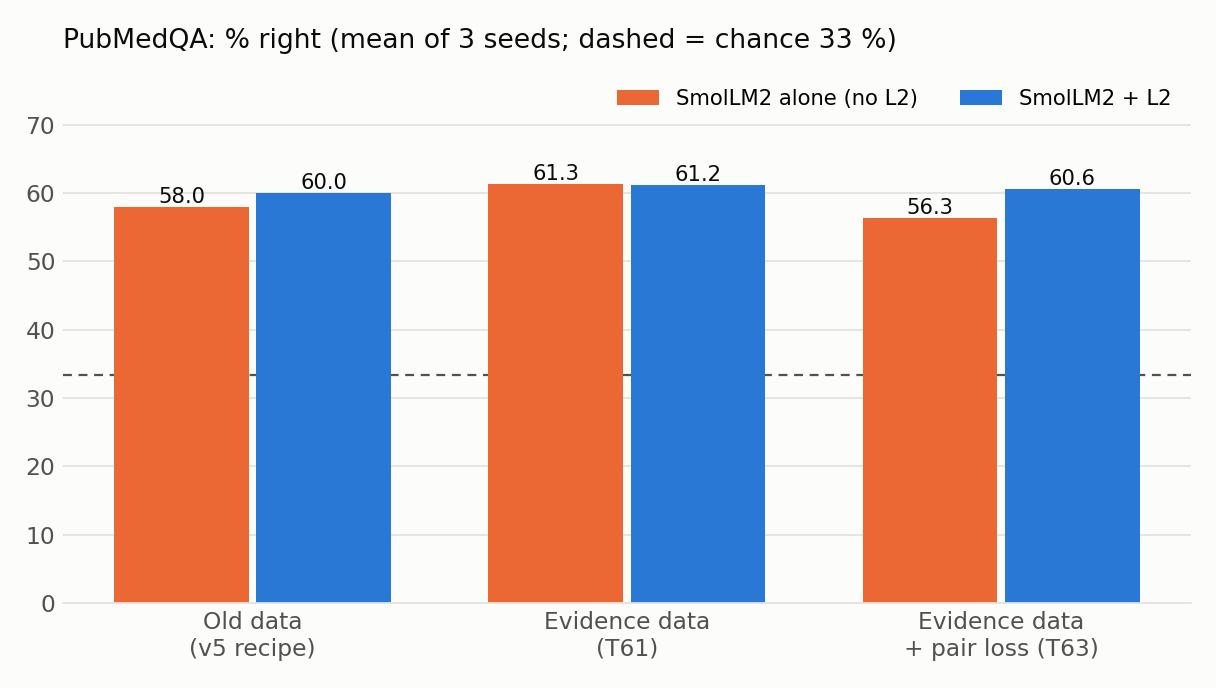
\includegraphics[width=0.86\linewidth]{../figures/update_1_pubmedqa.png}
\caption{PubMedQA accuracy (mean of three seeds). Orange: SmolLM2 alone; blue: SmolLM2 + L2; dashed: chance.}
\end{figure}

\begin{table}[H]
\centering\small
\begin{tabularx}{\linewidth}{@{}YrrR@{}}
\toprule
Training data & SmolLM2 alone & SmolLM2 + L2 & L2 minus alone [95\,\% CI]\\
\midrule
Old data (baseline / v5) & 58.0 & 60.0 & \textbf{+2.07} [+0.57, +3.73]\sig\\
Evidence data (evbase / ev5) & 61.3 & 61.2 & $-0.10$ [$-0.70$, +0.47]\\
Evidence + pair loss (pairbase / pair5) & 56.3 & 60.6 & \textbf{+4.27} [+3.10, +5.57]\sig\\
\bottomrule
\end{tabularx}
\caption{PubMedQA \% right.}
\end{table}

Against the old baseline (58.0\,\%), the evidence data gives \textbf{+3.30\sig} without L2 and +3.20\sig{} with L2; the 3-benchmark average rises by +1.25\sig{} and +1.22\sig{} (v5: +0.72\sig). MedMCQA and MedQA never change by more than $\pm0.5$ points (never starred); they stay near chance for a 135\,M model.

\subsection{Reasoning tests}

\begin{figure}[H]
\centering
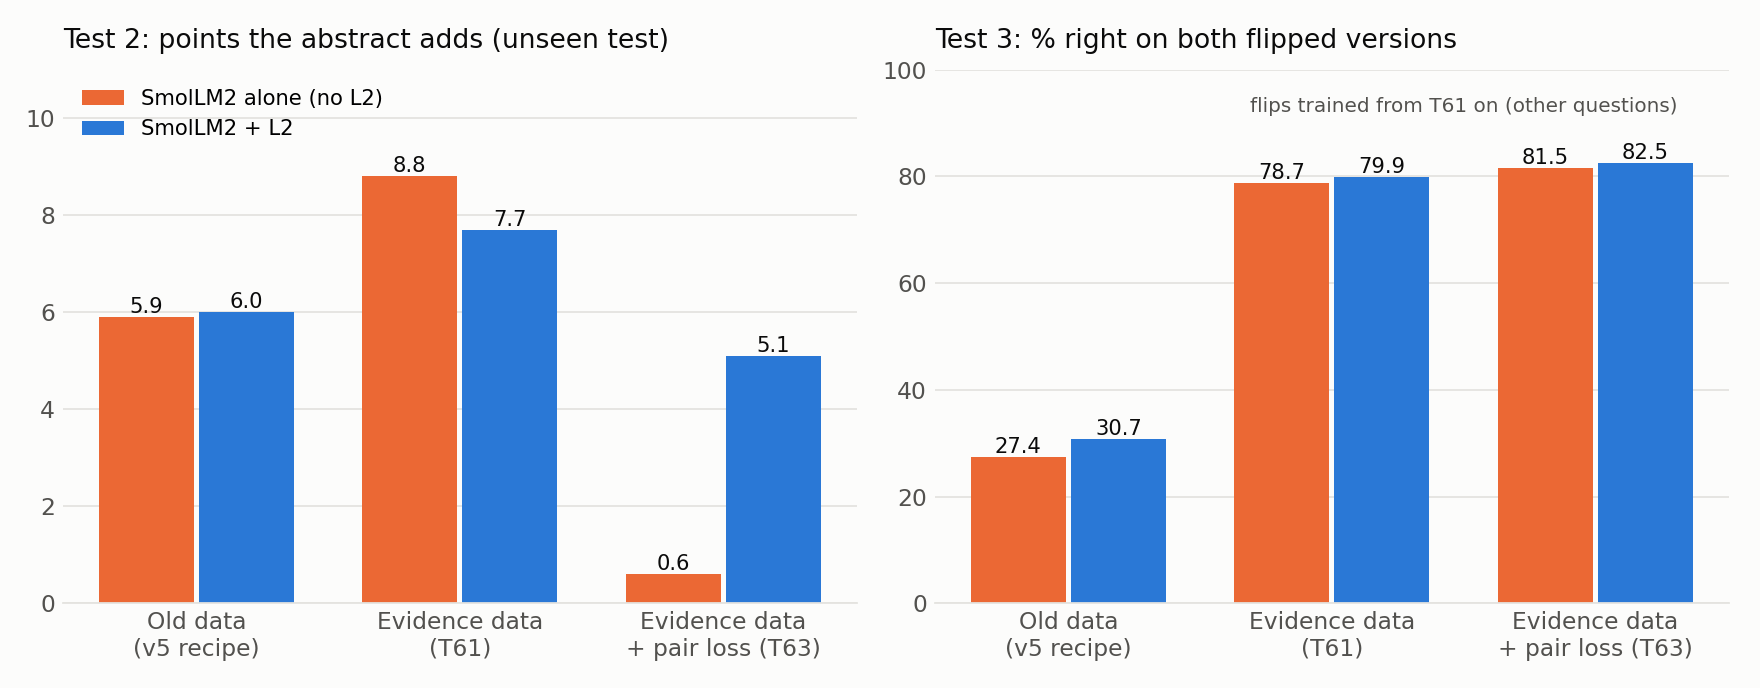
\includegraphics[width=\linewidth]{../figures/update_2_reasoning.png}
\caption{Left: test 2, points the abstract adds (unseen). Right: test 3, \% right on both flipped versions.}
\end{figure}

\begin{table}[H]
\centering\small
\begin{tabularx}{\linewidth}{@{}YRRR@{}}
\toprule
Model & Uses the abstract (test 2) & Follows flipped evidence (test 3) & Same answer on both versions\\
\midrule
baseline / v5 & 5.9 / 6.0 & 27.4\,\% / 30.7\,\% & 69.3\,\% / 65.7\,\%\\
evbase / ev5 & 8.8 / 7.7 & 78.7\,\% / 79.9\,\% & 13.8\,\% / 12.2\,\%\\
pairbase / pair5 & 0.6 / 5.1 & 81.5\,\% / 82.5\,\% & 14.0\,\% / 12.8\,\%\\
\bottomrule
\end{tabularx}
\caption{Reasoning tests 2 and 3.}
\end{table}

Test~3 jumps from about 27\,\% to about 80\,\% with the evidence data. This shows that the training worked; it is no longer an unseen test. The pair loss makes SmolLM2 alone almost stop using the abstract (0.6 points).

\subsection{What L2 adds on the same data}

\begin{figure}[H]
\centering
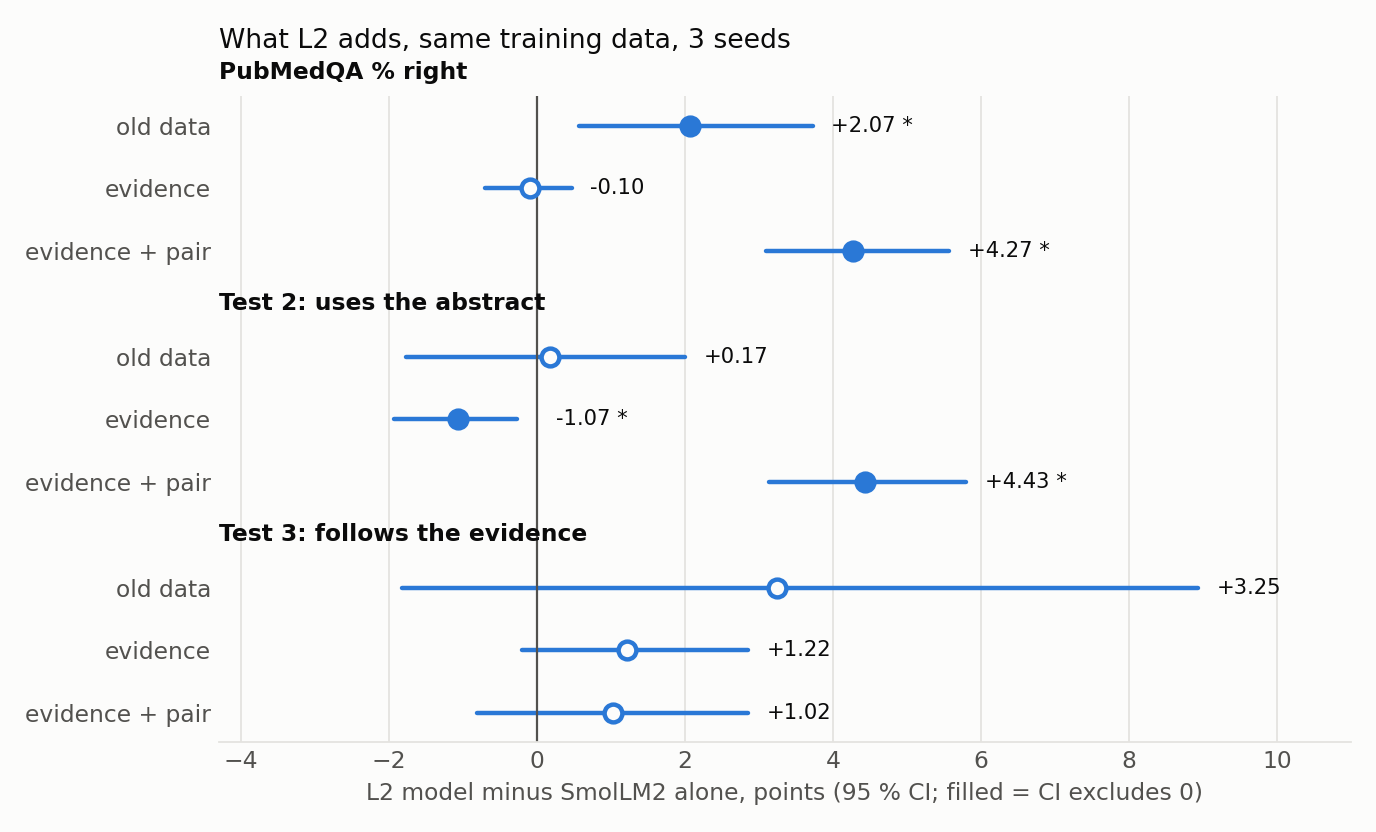
\includegraphics[width=0.82\linewidth]{../figures/update_4_l2_effect.png}
\caption{L2 minus SmolLM2 alone, same training data, with 95\,\% CIs. Filled dot: the interval excludes 0. Test 3 is never starred, so the decision rule is never met.}
\end{figure}

\begin{itemize}
  \item \textbf{Old data:} the gain is a preference (+11.0\sig{} more ``yes'' answers); tests 2 and 3 are not starred.
  \item \textbf{Evidence data:} L2 adds nothing and uses the abstract slightly \emph{less} ($-1.07$\sig).
  \item \textbf{Pair loss:} the first starred test-2 gain, on every seed (+4.8\sig{} / +5.8\sig{} / +2.7\sig). But it is measured against a baseline the pair loss damaged, test 3 is not starred (+1.02), and the L2-off test shows it is not L2's work.
\end{itemize}

\subsection{Switching L2 off at test time}

\begin{figure}[H]
\centering
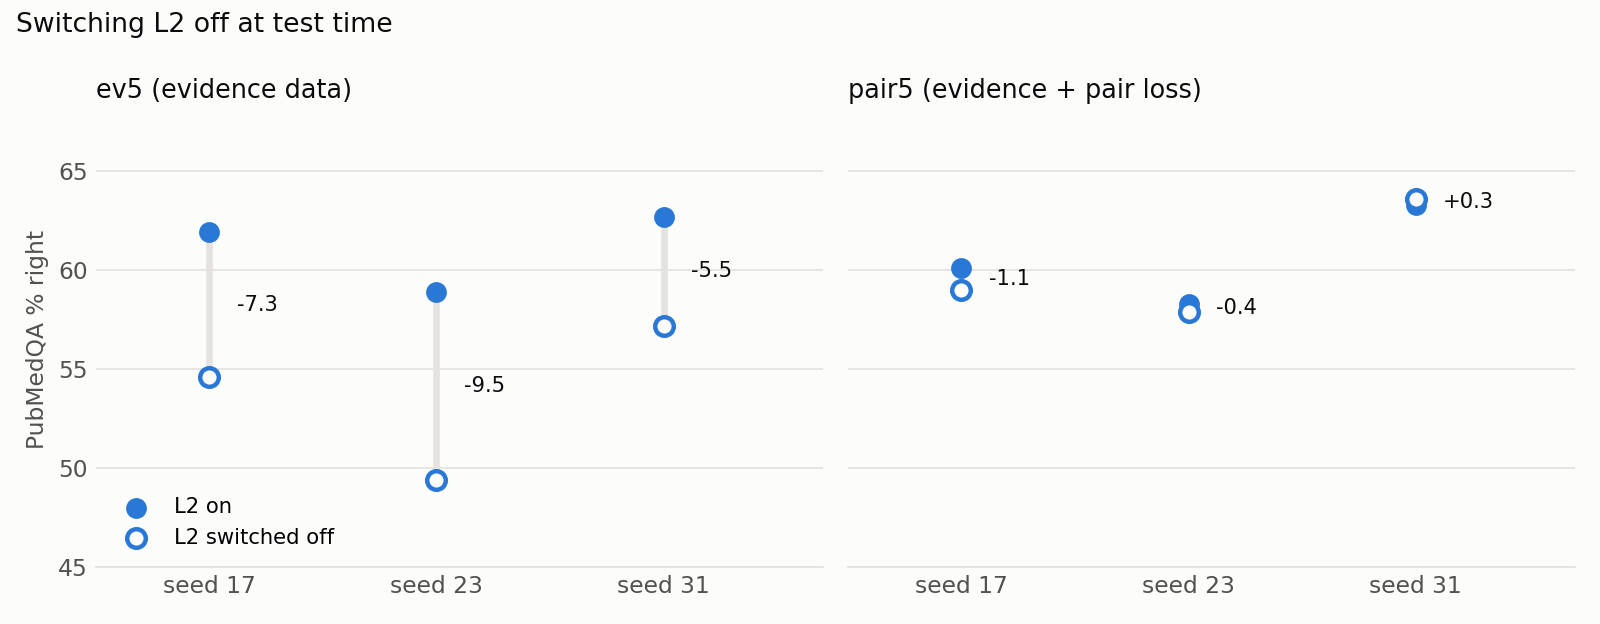
\includegraphics[width=0.92\linewidth]{../figures/update_5_l2_off.png}
\caption{PubMedQA per seed with L2 on (filled) and switched off (open).}
\end{figure}

\textbf{ev5 depends on L2} -- without it, PubMedQA drops by 5.5--9.5 points -- yet it is no better than the model trained without L2: SmolLM2 handed part of its own work to L2. \textbf{pair5 does not depend on L2} ($-1.1$ / $-0.4$ / +0.3 points; gate 0.015 against 0.027 for ev5). Its lead over pairbase sits in SmolLM2's own weights: training next to L2 kept the backbone from collapsing under the pair loss, but L2 does not compute the answer at test time.

\subsection{Answer preference}

\begin{figure}[H]
\centering
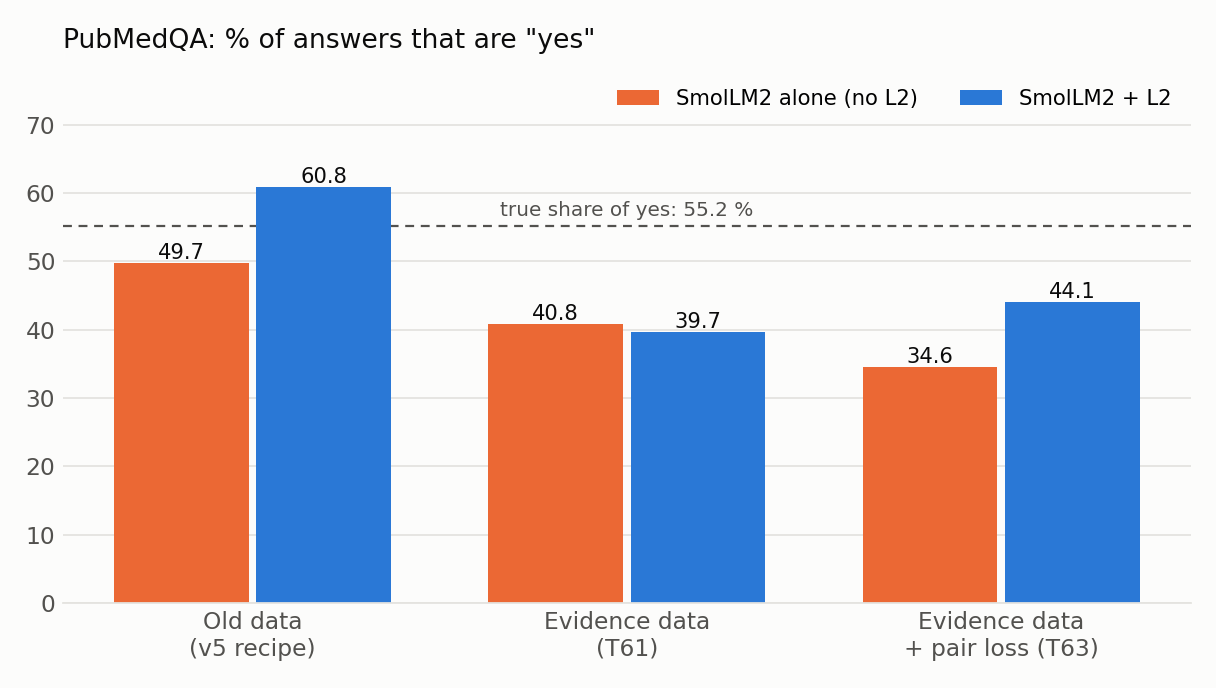
\includegraphics[width=0.86\linewidth]{../figures/update_3_preference.png}
\caption{Share of ``yes'' answers on PubMedQA; the dashed line is the true share (55.2\,\%).}
\end{figure}

v5 overshoots ``yes'' (60.8\,\%). The evidence-trained models under-say it ($\approx$ 40\,\%): they are right on 87--88\,\% of the true-no questions and 57--58\,\% of the true-yes ones. The pair loss pushes SmolLM2 alone further, to 34.6\,\%.

\subsection{Text generation}

\begin{table}[H]
\centering\small
\begin{tabularx}{\linewidth}{@{}YRR@{}}
\toprule
L2 minus alone, same data & Old data (v5) & Evidence data (ev5)\\
\midrule
MedQuAD perplexity & $-0.16$\,\%\sig & $-0.15$\,\%\sig\\
MedMCQA explanation perplexity & $-1.78$\,\%\sig & $-1.46$\,\%\sig\\
PubMedQA conclusion perplexity & $-0.45$\,\%\sig & +0.84\,\%\sig{} (worse)\\
\midrule
Generated: explanation ROUGE-L & +0.05 & +0.01\\
Generated: explanation names the right answer & $-0.67$ & $-0.83$\\
Generated: conclusion ROUGE-L & $-0.35$ & $-0.02$\\
\bottomrule
\end{tabularx}
\caption{Text measures. Upper block: how well the model predicts reference text; lower block: the text it writes itself.}
\end{table}

L2 lowers perplexity slightly (under 2\,\%, consistently across seeds), but \textbf{the text it writes is no better}: no generated-text measure differs significantly. The evidence data has the larger effect: explanation perplexity $-5.33$\,\%\sig{} without L2 and $-6.72$\,\%\sig{} with L2 against the old baseline, at the cost of PubMedQA conclusion perplexity (+11.7 / +12.7\,\%\sig{} worse, because less conclusion text is trained). The pair loss makes generated explanations worse: ROUGE-L $-1.99$\sig{} (pairbase) and $-3.15$\sig{} (pair5) against evbase.

% =====================================================================
\section{Discussion}

\subsection{Verdict on L2}

\begin{keybox}[title={Verdict},colframe=lorange,colback=lorange!6]
\textbf{L2 is not useful for this task and is not worth keeping.}
\begin{itemize}[leftmargin=1.2em]
  \item \textbf{Reasoning:} never shown; the pre-registered rule (starred gains on tests 2 and 3) was never met.
  \item \textbf{Accuracy:} its only fair gain (+2.07\sig{} on PubMedQA, old data) was a ``yes'' preference; with the evidence data it adds $-0.10$ points; MedMCQA and MedQA never moved.
  \item \textbf{Text generation:} perplexity drops by under 2\,\%, but the written text is no better.
  \item \textbf{Cost:} 19.6\,M extra parameters (+14.6\,\%); the model learns to lean on L2 without beating the model trained without it.
\end{itemize}
\end{keybox}

\subsection{A likely reason (interpretation)}

In v5, L2 only reshapes each token's final state (Section~\ref{sec:l2}); it has no access to evidence that SmolLM2 has not already encoded, and nothing downstream reads its output except the output layer. A module in this position can re-weight the final decision -- which is exactly the answer preference we measured -- but it has little room to add reasoning. The versions that let L2 read the text and sit inside the network (v3--v4) were not better either, so position alone does not explain the result. This interpretation is not separately tested.

\subsection{Limitations}
\begin{itemize}
  \item \textbf{Scale.} A 135\,M backbone stays near chance on MedMCQA and MedQA, so only PubMedQA can show differences.
  \item \textbf{Parameter matching.} The comparison is architecture-matched, not parameter-matched: the L2 arm has 19.6\,M more parameters and does more work per token. This favours L2, which strengthens the negative result.
  \item \textbf{Test 3 after T61.} Flipped conclusions are in the training data from T61 on (other questions); test 3 then measures training success, and test 2 is the unseen check.
  \item \textbf{Rule-based flips.} Negations are added or removed by a rule; some flipped sentences may be unnatural. The full list was written out for manual checking.
  \item \textbf{Labels.} \code{pqa\_artificial} labels are generated automatically; the benchmark (\code{pqa\_labeled}) uses expert labels.
  \item \textbf{Seeds.} Three seeds per model; intervals are computed over questions with the same resample in every seed.
\end{itemize}

% =====================================================================
\section{Conclusions}

What the thesis can claim:
\begin{enumerate}
  \item \textbf{The data finding.} The yes/no decision was never trained and the data was 92.8\,\% ``yes''. Training the decision from balanced and flipped evidence improves PubMedQA (+3.3\sig{} points) and the 3-benchmark average (+1.25\sig), raises following flipped evidence from 27\,\% to 80\,\%, and is cheaper to train.
  \item \textbf{The evaluation method.} Splitting accuracy by the true answer, ``uses the abstract'', the flipped-evidence test and the L2-off test turned an apparent +2-point ``reasoning'' gain into an answer preference. Accuracy alone would have hidden it.
  \item \textbf{A careful negative result for L2}, measured against a same-data baseline on three seeds with confidence intervals.
\end{enumerate}

\section{Questions for discussion}
\begin{enumerate}
  \item Should the thesis be framed as a careful negative result for L2, with the data finding and the evaluation method as the positive contributions?
  \item Stop experimenting and start writing, or run one more check (for example an unseen flipped-evidence format, since test 3 is now trained-like)?
  \item Final model: the proposal is the evidence-data recipe \textbf{without} L2 (evbase) -- it scores the same as ev5 with 19.6\,M fewer parameters.
\end{enumerate}

% =====================================================================
\appendix
\section{Glossary}

\begin{tabularx}{\linewidth}{@{}p{3.2cm}Y@{}}
\toprule
Term & Meaning\\
\midrule
T-numbers & entries in the project issue list (\code{07-Management/10\_Known\_Issues.md}); each is one problem or experiment\\
v-numbers & versions of the L2 design (v1 \dots{} v5)\\
baseline & SmolLM2 alone (no L2), old data\\
v5 & SmolLM2 + L2, old data; the final L2 model\\
evbase / ev5 & SmolLM2 alone / + L2, evidence data (T61)\\
pairbase / pair5 & the same two with evidence data + pair loss (T63)\\
trajectory & one of L2's four candidate versions of the token's state\\
gate $g$ & 576 numbers deciding how much of L2's output reaches the output layer; 0 = L2 off\\
perplexity & $\exp$ of the mean negative log-likelihood per token; lower is better\\
\sig & the 95\,\% confidence interval of a difference excludes 0\\
\bottomrule
\end{tabularx}

\section{Reproducibility}

\begin{itemize}
  \item Code: repository \code{Ekdant-LLM}, folder \code{09-Code} (\code{src/ekdant/sandbox.py} = L2, \code{model.py} = gate and wiring, \code{train\_gen.py} = training incl.\ \code{-{}-evidence} and \code{-{}-pair-loss}, \code{gen\_eval.py} = benchmarks and reasoning tests); 346 automated tests.
  \item Final L2 configuration: \code{configs/v5\_final.json} ($K=4$, 4 rounds, MLP ratio 4, pre-norm, 8 descent steps, $\eta=0.0625$, $\rho_{\min}=0.05$, mean readout, gate cap 1.0, L2 after the final norm).
  \item Training: \code{python -m ekdant.train -{}-task gen -{}-batch-size 8 -{}-grad-accum 4 -{}-epochs 1 -{}-ft-epochs 3} plus \code{-{}-variant baseline|sandbox}, \code{-{}-seed}, and \code{-{}-evidence} / \code{-{}-pair-loss 1.0} where stated.
  \item Run book with every command and raw result: \code{run.md}, sections A2, A3o--A3s, A7k--A7n.
\end{itemize}

% =====================================================================
\begin{thebibliography}{99}\small
\bibitem{smollm2} L.~B.~Allal et al. \emph{SmolLM2: When Smol Goes Big -- Data-Centric Training of a Small Language Model.} arXiv:2502.02737, 2025.
\bibitem{pubmedqa} Q.~Jin, B.~Dhingra, Z.~Liu, W.~Cohen, X.~Lu. \emph{PubMedQA: A Dataset for Biomedical Research Question Answering.} EMNLP-IJCNLP 2019.
\bibitem{medmcqa} A.~Pal, L.~K.~Umapathi, M.~Sankarasubbu. \emph{MedMCQA: A Large-scale Multi-Subject Multi-Choice Dataset for Medical domain Question Answering.} CHIL 2022, PMLR 174.
\bibitem{medqa} D.~Jin, E.~Pan, N.~Oufattole, W.-H.~Weng, H.~Fang, P.~Szolovits. \emph{What Disease Does This Patient Have? A Large-Scale Open Domain Question Answering Dataset from Medical Exams.} Applied Sciences 11(14):6421, 2021.
\bibitem{medquad} A.~Ben Abacha, D.~Demner-Fushman. \emph{A Question-Entailment Approach to Question Answering.} BMC Bioinformatics 20:511, 2019.
\bibitem{paircfr} X.~Qiu et al. \emph{PairCFR: Enhancing Model Training on Paired Counterfactually Augmented Data through Contrastive Learning.} ACL 2024.
\bibitem{kaushik} D.~Kaushik, E.~Hovy, Z.~C.~Lipton. \emph{Learning the Difference that Makes a Difference with Counterfactually-Augmented Data.} ICLR 2020.
\bibitem{lmeval} L.~Gao et al. \emph{A Framework for Few-Shot Language Model Evaluation (lm-evaluation-harness).} Zenodo, 2023.
\bibitem{rouge} C.-Y.~Lin. \emph{ROUGE: A Package for Automatic Evaluation of Summaries.} ACL Workshop Text Summarization Branches Out, 2004.
\bibitem{rmsnorm} B.~Zhang, R.~Sennrich. \emph{Root Mean Square Layer Normalization.} NeurIPS 2019.
\bibitem{bootstrap} B.~Efron, R.~J.~Tibshirani. \emph{An Introduction to the Bootstrap.} Chapman \& Hall, 1993.
\end{thebibliography}

\end{document}
